\documentclass[manuscript, 12pt]{copernicus}

\usepackage{amsmath}
\usepackage{graphicx}
\usepackage{booktabs}
\usepackage{siunitx}
\usepackage{natbib}
\usepackage{hyperref}

\title{When does cluster proximity matter? Mapping design regret across wind rose shape and neighbor distance}

\Author[1]{Julian}{Quick}
\Author[1]{Pierre-Elouan}{R\'ethor\'e}

\affil[1]{Technical University of Denmark, Department of Wind and Energy Systems, Roskilde, Denmark}

\correspondence{Julian Quick (juqu@dtu.dk)}

\runningtitle{Design regret across wind rose shape and neighbor distance}
\runningauthor{Quick and R\'ethor\'e}

\begin{document}

\maketitle

\begin{abstract}
Wind farms in emerging offshore clusters are typically designed before neighboring farms are fully specified.
This creates \emph{design regret}---the annual energy production (AEP) lost by optimizing a layout without accounting for neighbors that later appear.
Using a bilevel optimization framework in which greedy neighbor placement maximizes regret against a re-optimized target layout, we systematically map design regret across wind rose shape and neighbor distance.
Wind rose shape is parameterized using the two-parameter elliptical model of \citet{Hart2025}, spanning bidirectional-to-unidirectional and uniform-to-concentrated regimes.
We find that regret varies 7.8-fold across wind rose shape space, with the folding parameter (bidirectional vs.\ unidirectional character) as the dominant driver.
A novel \emph{regret cross-section}---the polar map of regret versus neighbor bearing and distance for a reference neighbor farm---reveals an ``ambush effect'': peak design vulnerability occurs at oblique angles to the dominant wind direction, not along it.
These results explain why an earlier case study of the Danish Energy Island found negligible design tradeoffs: its moderately diffuse, bidirectional wind rose sits in the low-regret region of shape space.
We conclude that inter-farm buffer distance requirements should be wind-rose-dependent, not uniform.
\end{abstract}

\introduction

Offshore wind farms are designed in isolation, but operate in clusters.
This mismatch costs energy: wakes from neighboring farms persist for tens of kilometers \citep{Platis2018, Schneemann2020}, yet each farm's layout is typically optimized without knowledge of what will be built nearby \citep{Quick2026omae}.
A recent case study of the Danish Energy Island cluster found negligible design tradeoffs from this ignorance \citep{Quick2026omae}, suggesting that inter-farm coordination may be unnecessary.
We show this conclusion is site-specific: it holds for the Danish Energy Island's moderately diffuse wind rose, but not for sites with concentrated, unidirectional wind climates---where the cost of designing in isolation can exceed 2\% of annual energy production.

In emerging North Sea clusters, farms are designed and permitted sequentially, often by different developers \citep{Fischereit2022}.
A target farm's layout is typically optimized before the characteristics of neighboring farms are fully known \citep{Quick2026omae}.
This creates a design problem under uncertainty: should the developer design the farm optimistically, assuming no neighbors (the \emph{liberal} scenario), or pessimistically, assuming neighbors will appear in the worst possible configuration (the \emph{conservative} scenario)?

We define \emph{design regret} as the AEP gap between these two strategies when evaluated under the same neighbor configuration:
\begin{equation}\label{eq:regret}
    \text{regret} = \text{AEP}_\text{cons}[\mathbf{x}^*_\text{cons}, \mathbf{n}] - \text{AEP}_\text{cons}[\mathbf{x}^*_\text{lib}, \mathbf{n}],
\end{equation}
where $\mathbf{x}^*_\text{cons}$ is the layout optimized with knowledge of neighbors $\mathbf{n}$, and $\mathbf{x}^*_\text{lib}$ is the layout optimized in isolation.
Both AEP evaluations include the neighbors' wakes, isolating the pure design effect.
A positive regret means the liberal designer would have chosen a better layout had they anticipated the neighbors.

\citet{Quick2026omae} applied this framework to the Danish Energy Island (DEI) cluster, examining nine real neighboring farms.
Surprisingly, they found negligible design regret---less than 0.2\% of AEP---for all neighbor configurations.
This raised a question: is design regret generally negligible for offshore wind clusters, or was this a property of the specific site?

We address this question by systematically varying the two factors most likely to govern regret: \emph{wind rose shape} and \emph{neighbor distance}.
Wind rose shape is parameterized using the elliptical model of \citet{Hart2025}, which separates directional concentration (parameter $a$) from bidirectional character (parameter $f$).
This enables a controlled sweep across the full space of plausible wind climates.

We introduce the \emph{regret cross-section}: a polar map showing design regret as a function of neighbor bearing and distance for a standardized reference neighbor farm.
This diagnostic tool reveals an ``ambush effect''---peak vulnerability occurs at oblique angles to the dominant wind direction, not along it---because the liberal layout is already adapted to the dominant direction and therefore resilient to aligned neighbors.

The paper is organized as follows.
Section~\ref{sec:methods} describes the bilevel optimization framework, wind rose parameterization, and experimental design.
Section~\ref{sec:results} presents three sets of results: the wind rose shape sweep, the buffer distance analysis, and the regret cross-sections.
Section~\ref{sec:discussion} discusses the physical mechanisms, practical implications, and limitations.

\section{Methods}\label{sec:methods}

\subsection{Bilevel optimization framework}

Design regret requires solving a bilevel optimization problem.
The \emph{inner} problem optimizes the target farm layout for a given neighbor configuration, and the \emph{outer} problem searches for the neighbor configuration that maximizes regret.

\subsubsection{Inner layout optimization}

The target farm layout is optimized using stochastic gradient descent (SGD) with boundary and spacing constraints, following \citet{Quick2023sgd}.
The objective is to maximize AEP:
\begin{equation}
    \max_{\mathbf{x}, \mathbf{y}} \; \text{AEP}(\mathbf{x}, \mathbf{y}, \mathbf{n}) = \sum_{k=1}^{N_d} w_k \sum_{i=1}^{N_t} P_i(u_k, \theta_k, \mathbf{x}, \mathbf{y}, \mathbf{n}) \cdot 8760,
\end{equation}
where $w_k$ are directional frequency weights, $P_i$ is the power of turbine $i$ under wind condition $k$, and $\mathbf{n}$ represents neighbor turbine positions.
Spacing constraints ($\|\mathbf{x}_i - \mathbf{x}_j\| \geq N_D D$, with $N_D = 4$) and boundary constraints are enforced via penalty terms.

To mitigate local optima, we employ $K = 5$ random restarts per evaluation:
\begin{enumerate}
    \item Start 0: regular grid initialization inside the target boundary.
    \item Start 1: the liberal layout (optimized without neighbors).
    \item Starts 2--4: random positions sampled uniformly inside the boundary polygon via rejection sampling.
\end{enumerate}
The best layout (highest AEP) is retained.
Including the liberal layout as a restart guarantees non-negative regret by construction, since the conservative optimization can always recover at least the liberal layout's performance.

The wake simulation uses the Bastankhah--Port\'e-Agel Gaussian deficit model \citep{Bastankhah2014} with wake expansion coefficient $k = 0.04$ and root-sum-of-squares superposition.
The simulation is implemented in JAX \citep{jax2018github}, enabling automatic differentiation through the entire wake model and SGD loop.

\subsubsection{Outer adversarial search: greedy grid placement}\label{sec:greedy}

For the wind rose shape sweep, neighbors are placed sequentially using a greedy grid search.
At each step, a discrete grid of candidate positions is constructed outside the target farm boundary (5$D$ spacing, 50$D$ extent).
Each candidate is screened by the AEP loss it inflicts on the liberal layout (cheap forward evaluation), and the top 10 candidates undergo full $K$-start inner optimization.
The candidate producing the highest regret is placed, and the process repeats.
This greedy approach is computationally efficient: all 10 candidates $\times$ 5 starts = 50 inner optimizations are parallelized on GPU via \texttt{vmap}.

\subsubsection{Regret cross-section: reference farm placement}\label{sec:cross-section}

For the regret cross-section analysis, we replace the greedy adversarial search with a controlled experiment: a standardized reference neighbor farm---a 5$\times$5 grid of 25 turbines at 7$D$ spacing---is placed at each combination of 24 bearings ($15°$ steps) and 7 distances (5, 10, 15, 20, 30, 40, 60$D$), yielding 168 evaluations per wind rose.
At each position, the target farm is re-optimized with $K = 5$ starts.
This produces a polar map of regret versus bearing and distance, analogous to a radar cross-section \citep{rcs_analogy}: it characterizes the target farm's directional vulnerability to neighbors.

\subsection{Wind rose parameterization}\label{sec:edrose}

Wind rose shape is parameterized using the elliptical model of \citet{Hart2025}, implemented in the \texttt{edrose} package.
The model describes the directional frequency distribution with three parameters:
\begin{itemize}
    \item $a$: shape parameter controlling directional concentration. $a = 1/\sqrt{\pi} \approx 0.564$ yields a uniform distribution; larger values concentrate probability along the prevailing direction.
    \item $f$: folding parameter in $[0, 1]$ controlling bidirectionality. $f = 0$ produces a symmetric bidirectional distribution (equal probability from opposite directions); $f = 1$ is fully unidirectional.
    \item $\theta_\text{prev}$: prevailing wind direction (fixed at $270°$ in this study).
\end{itemize}

This decomposition is well-suited to our problem because concentration and bidirectionality have distinct physical mechanisms for generating design regret.
Concentration creates narrow wake corridors that the liberal layout may not anticipate, while high folding ensures those corridors are consistently active from one direction rather than split between two.

We sweep $a \in \{0.3, 0.4, 0.5, 0.6, 0.7, 0.8, 0.9\}$ and $f \in \{0.0, 0.25, 0.5, 0.75, 1.0\}$, yielding 35 combinations spanning the full range from uniform/bidirectional to concentrated/unidirectional wind climates.

\subsection{Target farm configuration}

The target farm uses the boundary polygon of the Danish Energy Island tender area (dk0w), with 50 IEA 15\,MW reference turbines ($D = 240$\,m, hub height 150\,m) initialized on a regular grid at 4$D$ spacing.
The polygon spans approximately 33\,km north--south and 19\,km east--west.
All wind conditions use a constant wind speed of 9\,m\,s$^{-1}$; directional frequency is controlled by the edrose parameterization.

\subsection{Buffer distance}

The \emph{buffer distance} defines the minimum separation between the target farm boundary and the nearest neighbor position.
In the baseline configuration, the buffer is 2$D$ (480\,m).
We additionally sweep buffer distances of 10$D$ (2.4\,km), 20$D$ (4.8\,km), and 40$D$ (9.6\,km) for three representative wind roses.

\section{Results}\label{sec:results}

\subsection{Contrasting extremes: concentrated unidirectional vs.\ moderate bidirectional}

Before presenting the full parameter sweep, we contrast the two extreme cases to build intuition.

\paragraph{High-regret case ($a = 0.9$, $f = 1.0$).}
This concentrated, unidirectional wind rose focuses nearly all energy along the $270°$ (westerly) direction.
The greedy adversary places neighbors in a tight line upwind, exploiting the narrow wake corridor.
After 30 neighbors, design regret reaches 94.6\,GWh---2.4\% of the liberal AEP.
The conservative layout adapts by shifting turbines laterally to partially escape the wake corridor, but the polygon boundary limits this freedom.

\paragraph{Low-regret case ($a = 0.5$, $f = 0.0$).}
This moderately concentrated, bidirectional rose distributes energy roughly equally between $270°$ and $90°$.
Neighbors placed upwind from one direction are downwind from the other, diluting their impact.
The greedy adversary struggles to find high-regret positions; after 30 neighbors, regret is only 12.2\,GWh---0.3\% of AEP.
The layout requires minimal adaptation because no single direction dominates.

\subsection{Wind rose shape space}\label{sec:results-shape}

Figure~\ref{fig:edrose_heatmap} shows design regret across the full $(a, f)$ parameter space.
Regret varies 7.8-fold, from 12.2\,GWh ($a = 0.5$, $f = 0.0$) to 94.6\,GWh ($a = 0.9$, $f = 1.0$).

The folding parameter $f$ is the dominant driver.
Mean regret increases monotonically with $f$: from 49.6\,GWh at $f = 0.0$ (bidirectional) to 82.4\,GWh at $f = 1.0$ (unidirectional).
The concentration parameter $a$ has a weaker, non-monotonic effect: moderate concentration ($a \approx 0.5$) minimizes regret when combined with bidirectionality, but increases regret at high folding.

The Danish Energy Island wind rose, when fitted with the elliptical model, has approximately $a \approx 0.64$ and $f \approx 0.38$---firmly in the low-regret region.
This explains why \citet{Quick2026omae} found negligible design tradeoffs: the DEI wind rose is moderately concentrated and nearly bidirectional, the combination that produces the smallest design regret.

\begin{figure}
    \centering
    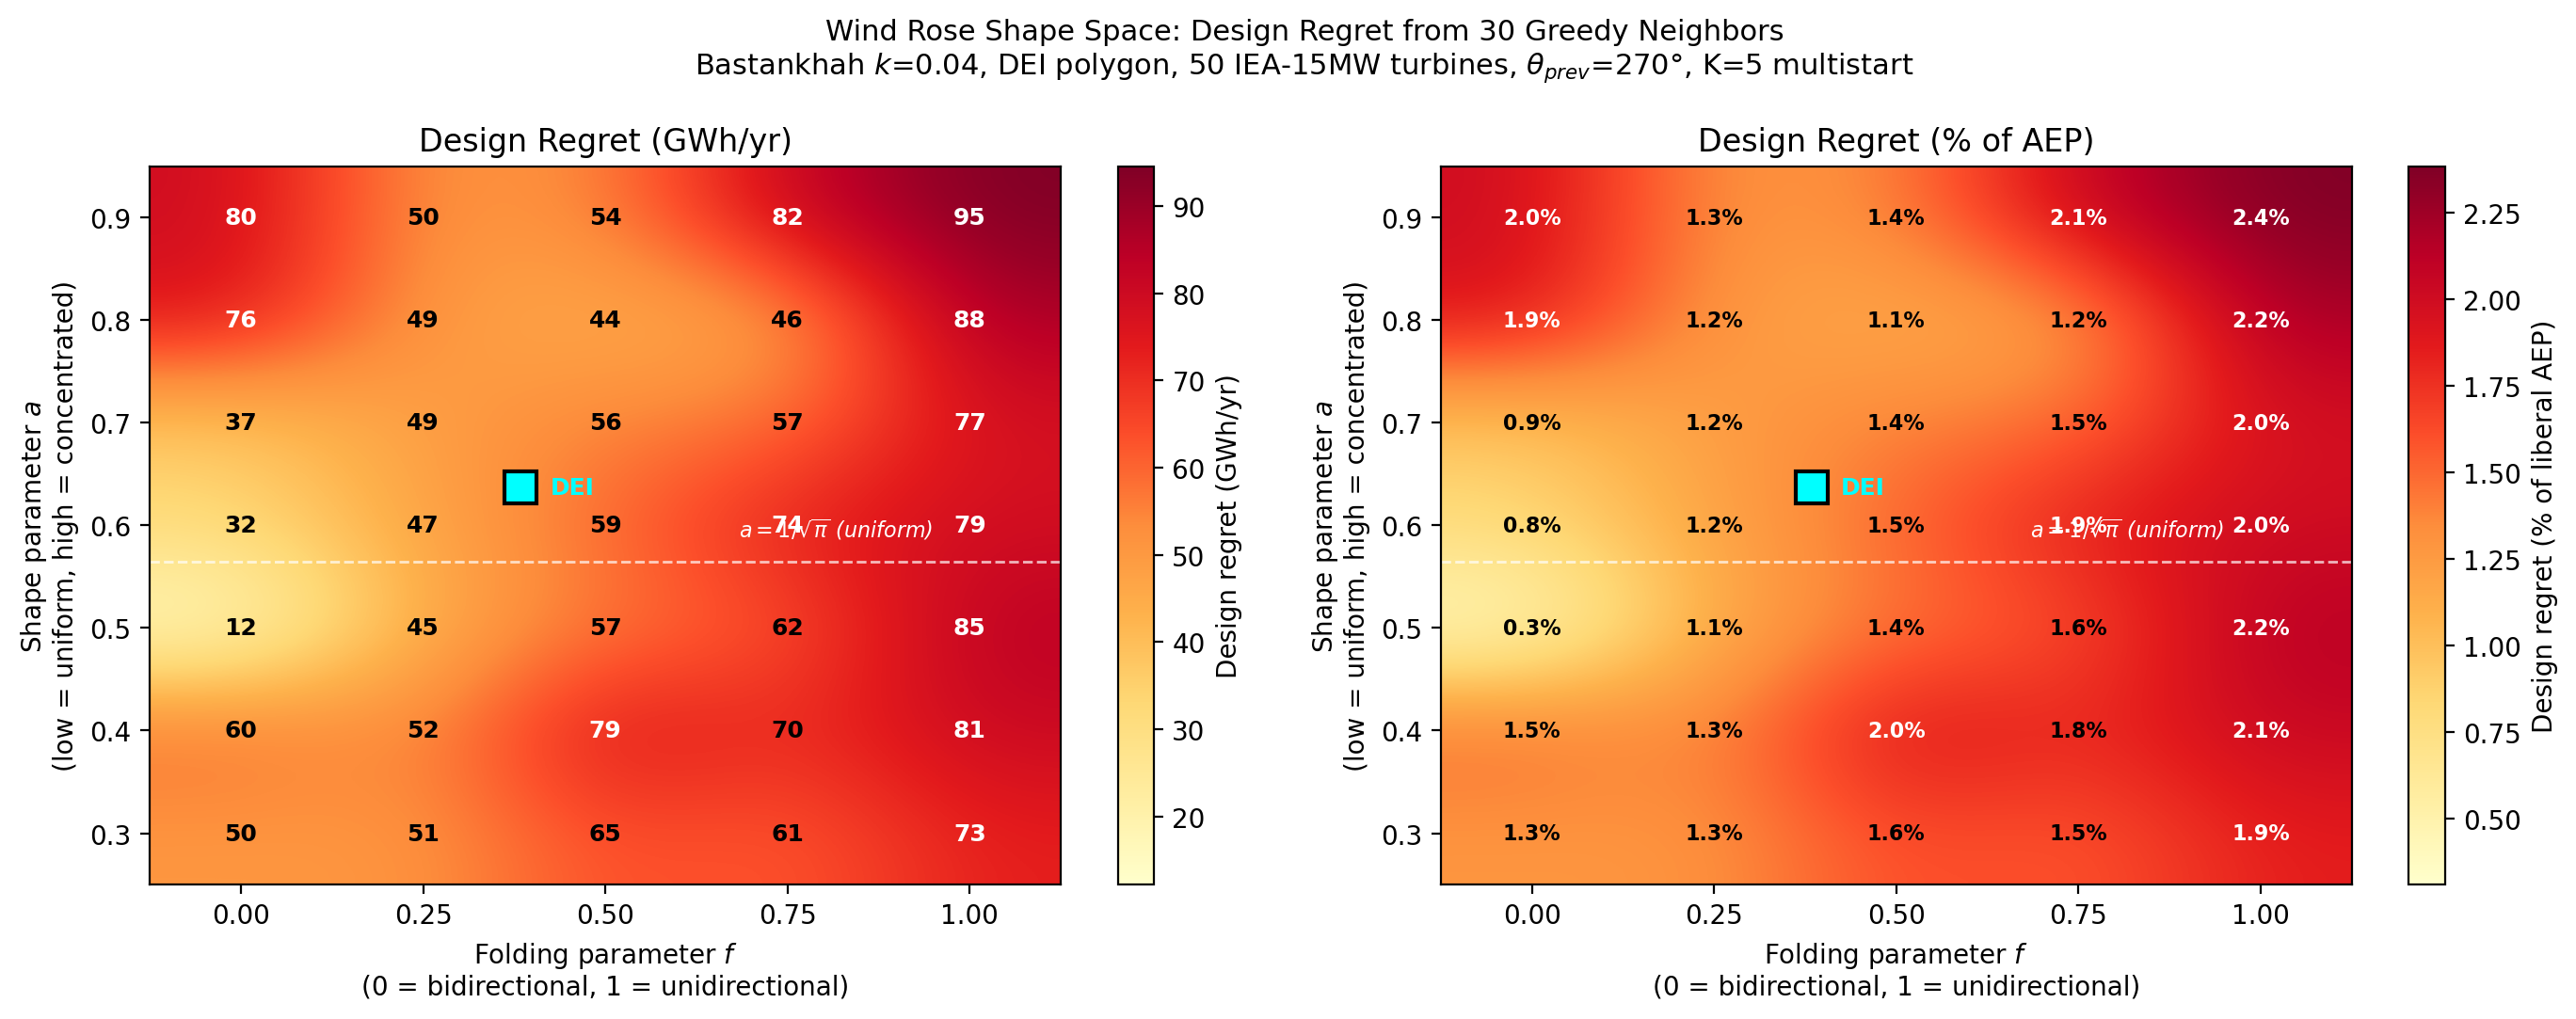
\includegraphics[width=\textwidth]{figures/edrose_heatmap.png}
    \caption{Design regret across the elliptical wind rose shape space $(a, f)$ for 30 greedy adversarial neighbors.
    Left: absolute regret (GWh/yr).
    Right: regret as percentage of liberal AEP.
    The dashed line marks $a = 1/\sqrt{\pi}$ (uniform distribution).
    Folding ($f$, bidirectional $\to$ unidirectional) is the dominant driver.
    The approximate location of the Danish Energy Island wind rose is indicated.}
    \label{fig:edrose_heatmap}
\end{figure}

\subsection{Buffer distance decay}\label{sec:results-buffer}

Figure~\ref{fig:buffer_decay} shows how regret decays with buffer distance for three representative wind roses.

For the concentrated unidirectional case ($a = 0.9$, $f = 1.0$), regret halves from 94.6\,GWh to 47.4\,GWh when the buffer increases from 2$D$ to 10$D$ (2.4\,km), and continues declining to 14.4\,GWh at 40$D$ (9.6\,km)---still 15\% of the zero-buffer value.

The mid-range case ($a = 0.7$, $f = 0.5$) exhibits a ``cliff'': regret holds steady from 2$D$ to 10$D$ (55.5 to 43.8\,GWh), then drops sharply at 20$D$ to 15.7\,GWh.

The bidirectional case ($a = 0.5$, $f = 0.0$) is essentially flat: regret remains near 12--13\,GWh regardless of buffer distance, dropping only at 40$D$.
For this wind rose, buffer distance is irrelevant because regret is already negligible.

These results demonstrate that a single buffer distance standard is inefficient: concentrated unidirectional sites need large buffers (30--40$D$, 7--10\,km), while bidirectional sites require none.

\begin{figure}
    \centering
    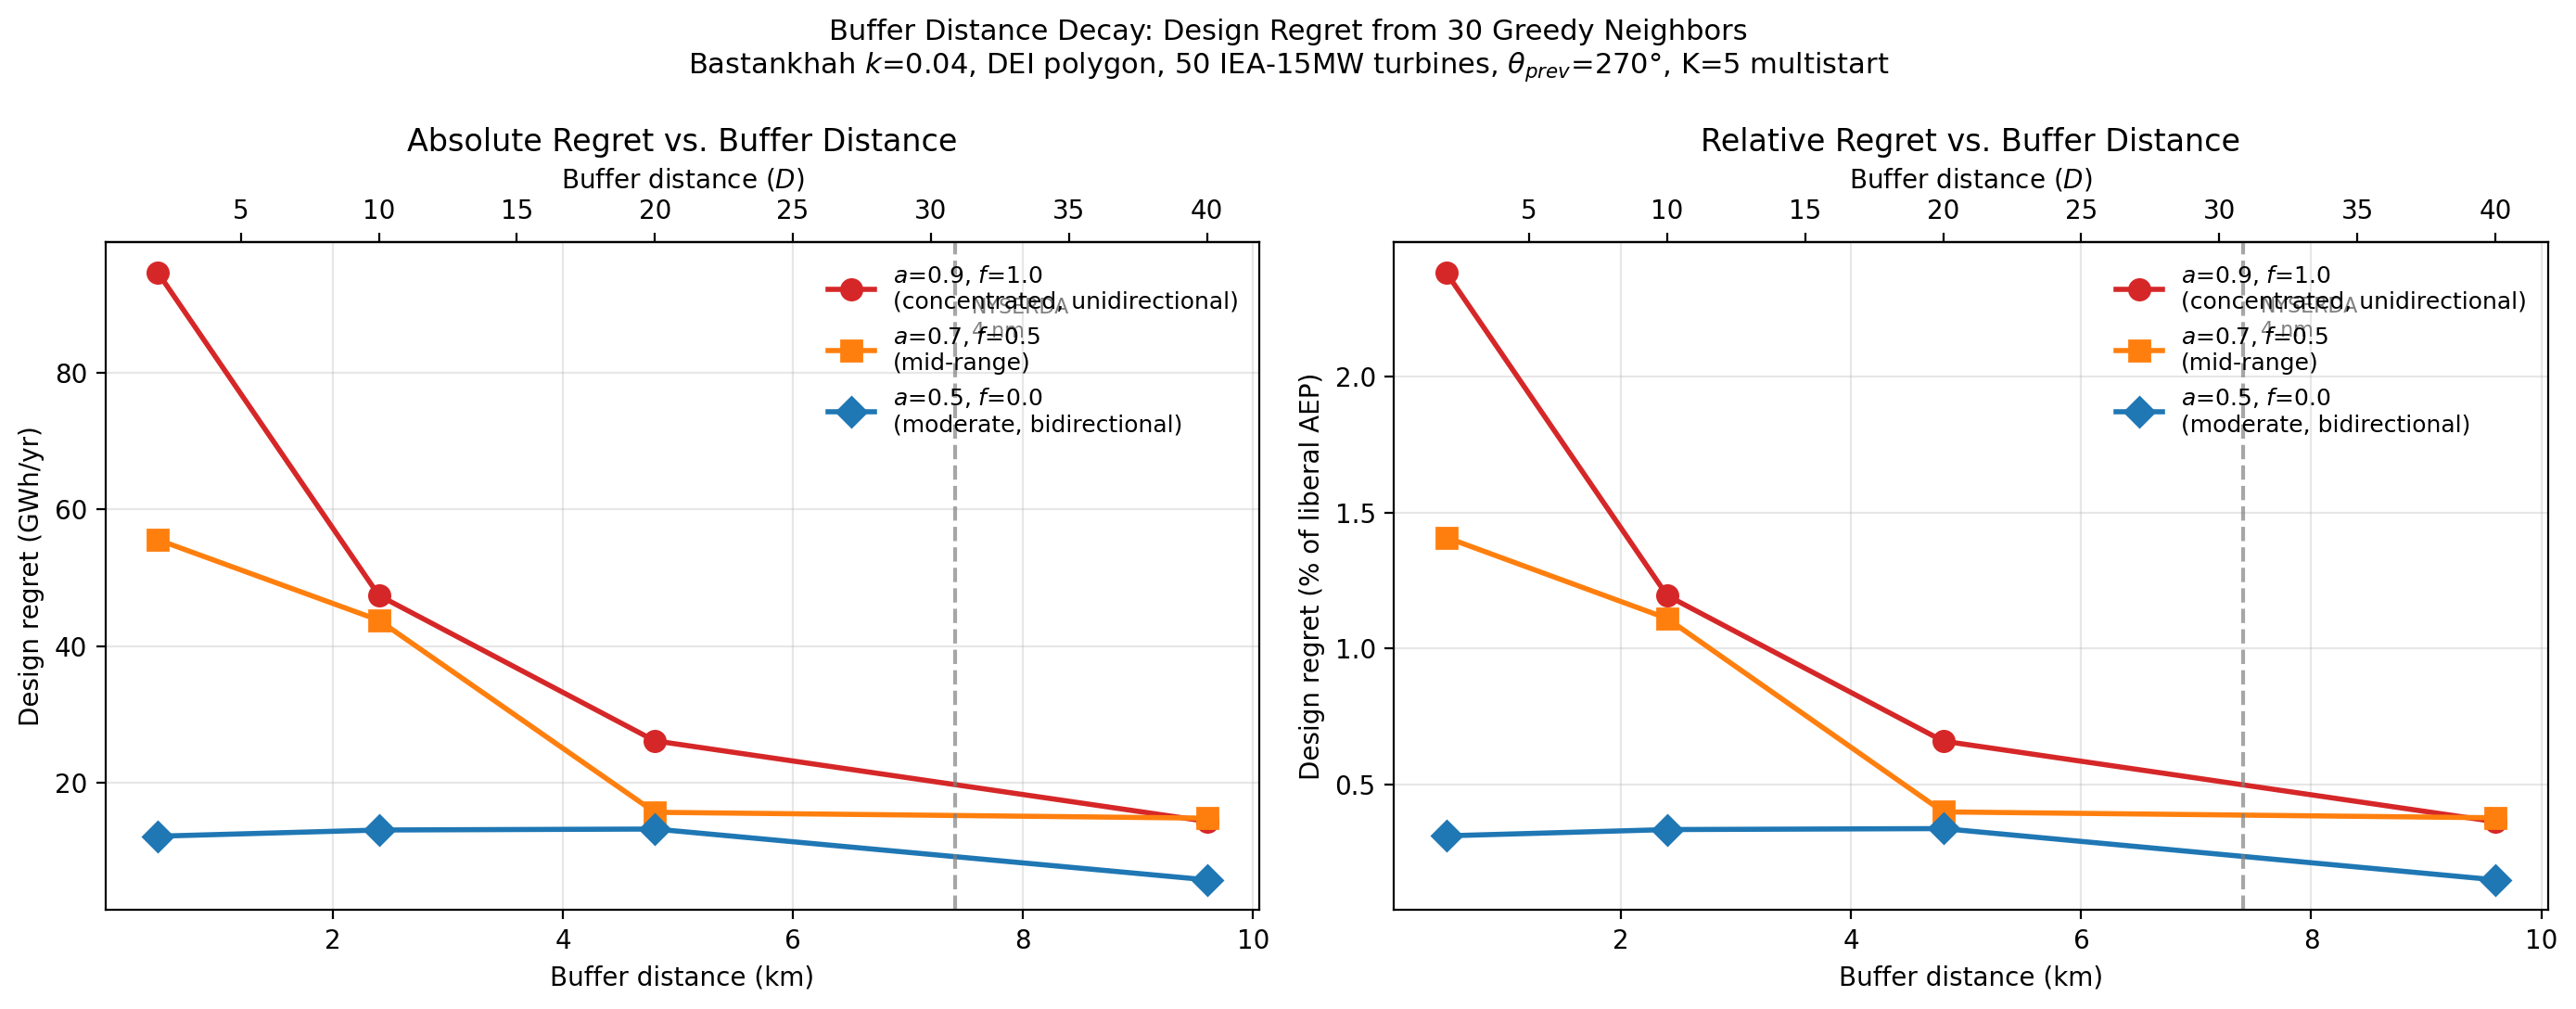
\includegraphics[width=\textwidth]{figures/buffer_decay.png}
    \caption{Design regret vs.\ buffer distance for three representative wind roses.
    The vertical dashed line marks the NYSERDA-recommended 4\,nm (7.4\,km) inter-farm spacing.
    Decay rate depends strongly on wind rose shape.}
    \label{fig:buffer_decay}
\end{figure}

\subsection{Regret cross-sections: the ambush effect}\label{sec:results-xsec}

Figure~\ref{fig:cross_section} presents regret cross-sections for five wind roses: the DEI empirical rose and four corners of the $(a, f)$ space.
Each panel shows regret as a function of neighbor bearing (angular position) and distance from the target farm centroid, with the corresponding wind rose shown as an inset.

The most striking finding is that peak regret does not occur at the bearing aligned with the dominant wind direction.
For the concentrated unidirectional case ($a = 0.9$, $f = 1.0$, dominant direction $270°$), the maximum regret occurs at bearing $105°$---nearly opposite and slightly offset from the dominant direction---at 5$D$ distance.
The DEI case peaks at $225°$, a southwesterly bearing offset from the dominant westerly direction.

We term this the ``ambush effect'': the liberal layout is already designed to perform well under the dominant wind direction.
Neighbors aligned with that direction cause wake losses, but the liberal layout is partly pre-adapted to handle them.
Off-axis neighbors exploit the layout's ``blind spots''---directions the liberal optimizer did not prioritize.

The moderate unidirectional case ($a = 0.5$, $f = 1.0$) shows the highest relative regret (3.61\% of AEP) at bearing $30°$ and 20$D$ distance, confirming that moderate concentration with strong folding creates the most vulnerable layouts.
The bidirectional case ($a = 0.5$, $f = 0.0$) has the lowest peak regret (1.92\%) and the most diffuse cross-section, consistent with its low vulnerability.

\begin{figure}
    \centering
    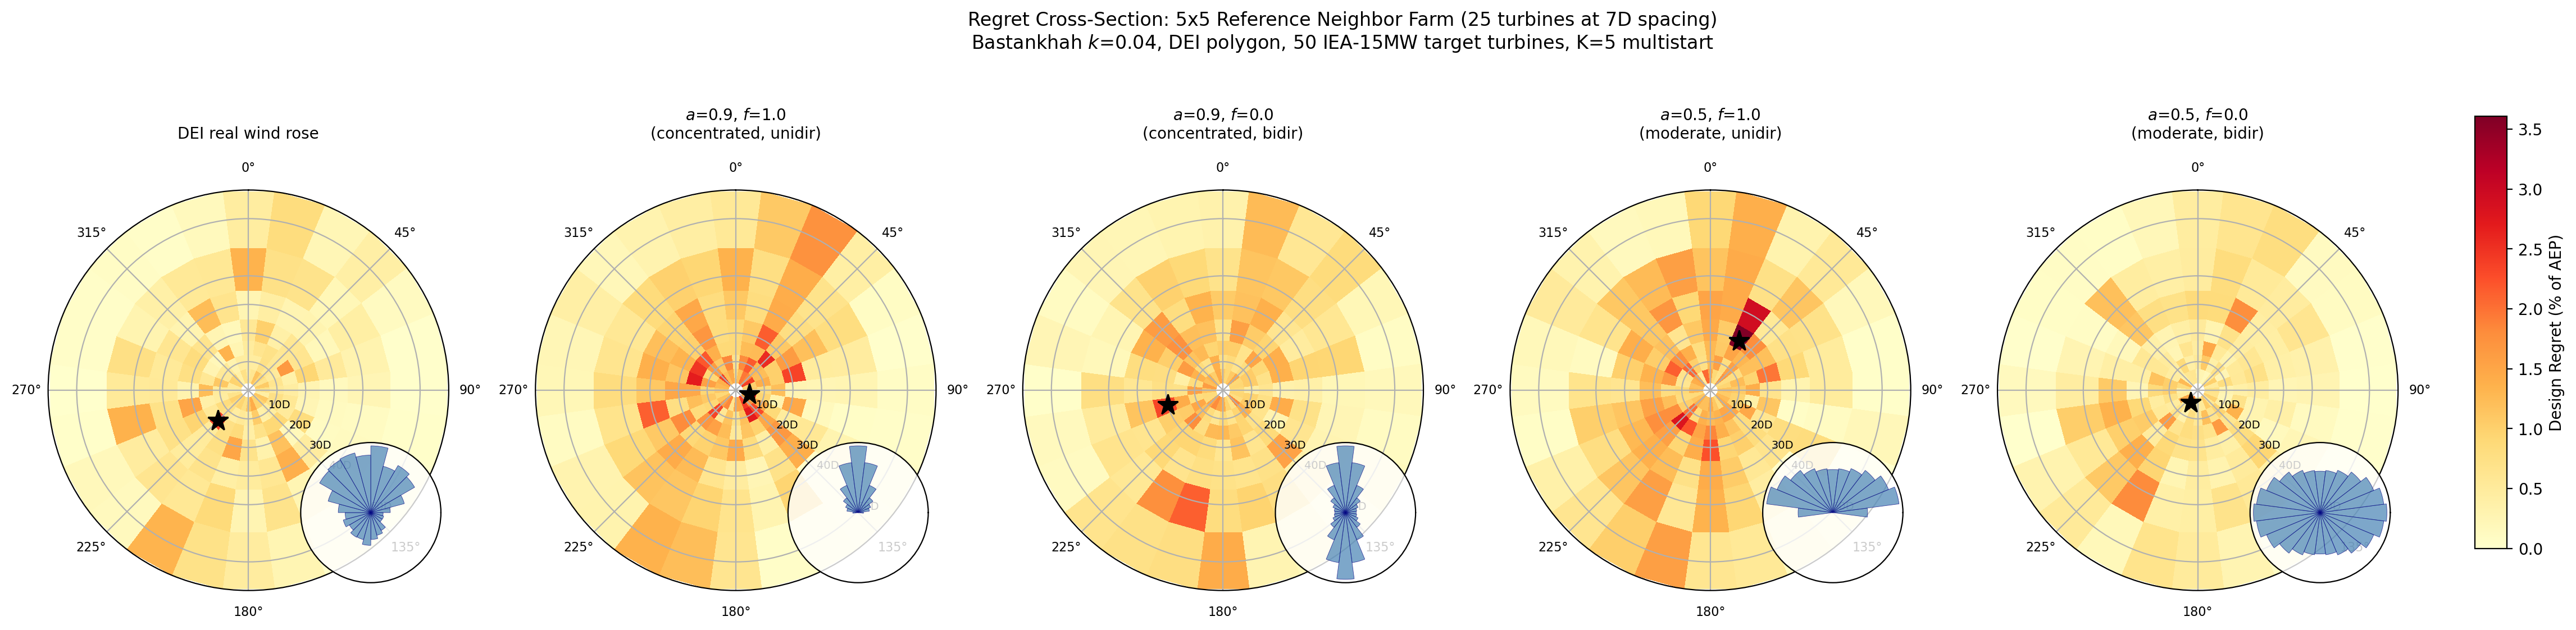
\includegraphics[width=\textwidth]{figures/cross_section.png}
    \caption{Regret cross-sections for five wind roses.
    Each polar panel shows design regret (\% of AEP) as a function of neighbor bearing and distance ($D$) for a 5$\times$5 reference farm.
    Stars mark peak regret positions.
    Wind rose insets show the corresponding directional frequency distribution.
    The ``ambush effect'' is visible: peak regret occurs at oblique angles to the dominant wind direction (270°), not along it.}
    \label{fig:cross_section}
\end{figure}

\subsection{Regret saturation with number of neighbors}

Figure~\ref{fig:saturation} shows how regret grows as greedy adversarial neighbors are placed sequentially.
For the Bastankhah unidirectional case, regret grows steeply for the first 30--50 neighbors, then plateaus near 270\,GWh after approximately 100 neighbors.
This confirms that 30 greedy neighbors (used in the wind rose shape sweep) capture the majority of the achievable regret, while the 200-neighbor runs reveal the saturation behavior.

\begin{figure}
    \centering
    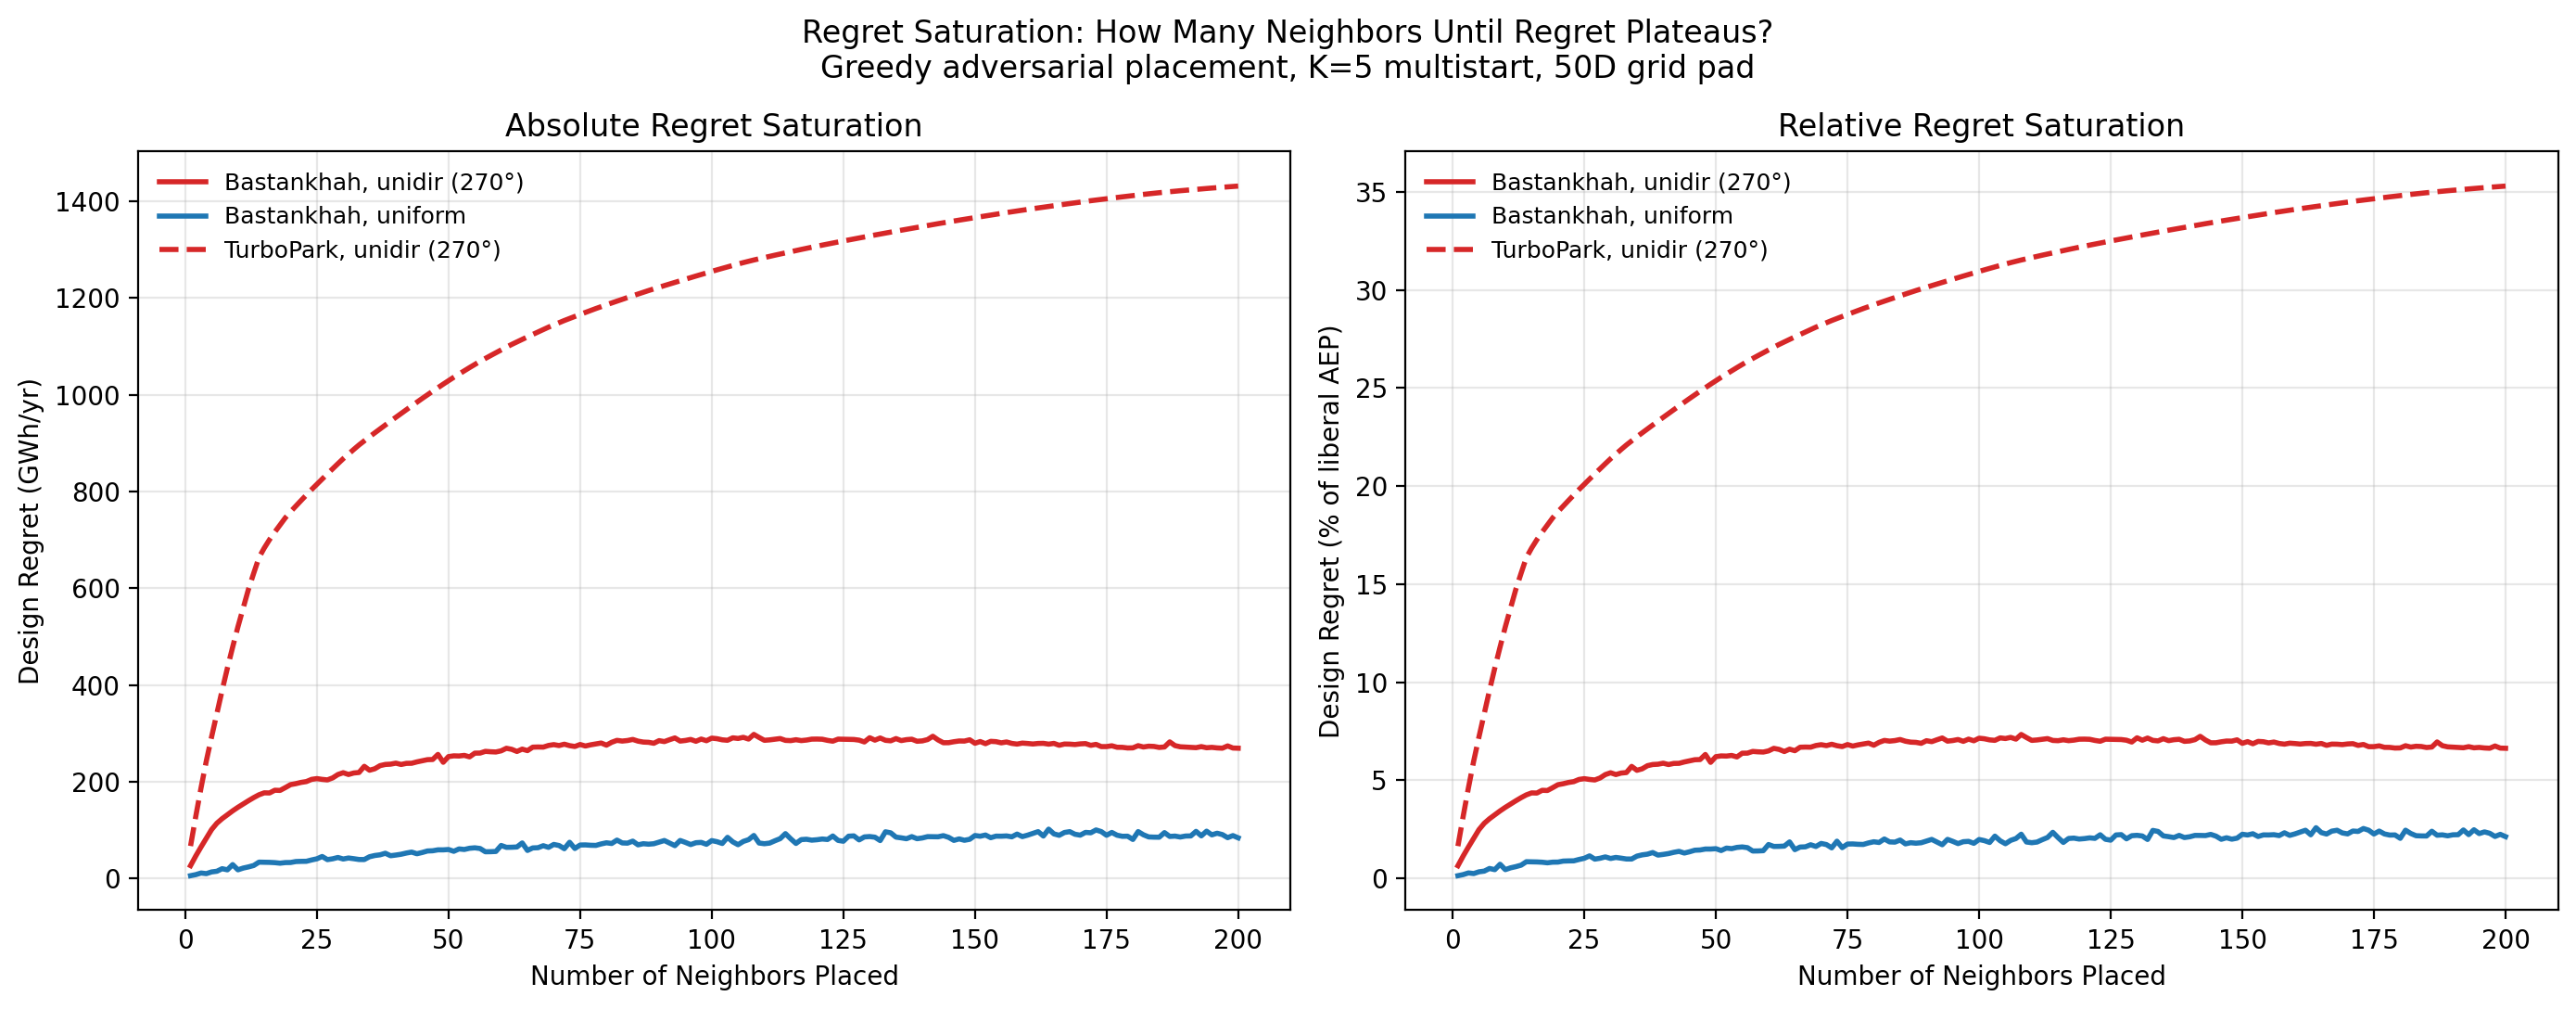
\includegraphics[width=\textwidth]{figures/saturation_curves.png}
    \caption{Regret vs.\ number of greedily placed neighbors for three configurations.
    Regret saturates as the most impactful positions are occupied first.
    The 30-neighbor mark (used in the wind rose sweep) captures the initial growth phase.}
    \label{fig:saturation}
\end{figure}

\subsection{Wake model sensitivity}

To assess robustness, we compare the Bastankhah Gaussian deficit ($k = 0.04$) with the TurbOPark model ($A = 0.04$, ambient TI $= 0.06$) for 30 greedy neighbors under unidirectional and uniform wind roses (Table~\ref{tab:wake_model}).
TurbOPark produces 4--10$\times$ higher absolute regret than Bastankhah, consistent with its wider, longer wakes driven by turbulence-intensity-dependent expansion.
However, the qualitative pattern---unidirectional $\gg$ uniform---is preserved across both models, suggesting that the wind rose shape conclusions are robust to wake model choice.

\begin{table}
    \centering
    \caption{Design regret (GWh/yr) for 30 greedy neighbors under two wake deficit models and two wind roses.}
    \label{tab:wake_model}
    \begin{tabular}{lcc}
        \toprule
        & Unidirectional ($270°$) & Uniform (24 dirs) \\
        \midrule
        Bastankhah ($k = 0.04$) & 212.9 & 30.4 \\
        TurbOPark ($A = 0.04$) & 818.3 & 164.5 \\
        \bottomrule
    \end{tabular}
\end{table}

\section{Discussion}\label{sec:discussion}

\subsection{The ambush effect: physical mechanism}

The ambush effect arises from an asymmetry between wake losses and layout adaptability.
When a neighbor appears along the dominant wind direction, the liberal layout---already optimized for that direction---has turbines positioned to partially mitigate wake interference.
The conservative layout can improve further, but the marginal gain is small because the liberal design is already well-adapted.

When a neighbor appears at an oblique angle, the liberal layout has no such pre-adaptation.
The wake corridor from an off-axis neighbor cuts across the farm at an angle the optimizer never considered.
The conservative layout can rearrange turbines to dodge this corridor, producing a larger gap between conservative and liberal AEP---larger regret.

This mechanism explains why bidirectional wind roses produce low regret: the liberal layout must accommodate two opposing directions, making it inherently more robust to neighbors from any bearing.
A unidirectional rose, by contrast, allows the liberal optimizer to specialize the layout for a single direction, creating blind spots in all other directions.

\subsection{Practical implications}

\subsubsection{Buffer distance policy}

Current inter-farm buffer distance standards, such as the NYSERDA-recommended 4\,nm (7.4\,km $\approx$ 31$D$), treat all sites equally.
Our results show this is inefficient: sites with bidirectional wind roses need no buffer (regret is negligible at any distance), while sites with concentrated unidirectional roses may need 40$D$+ (9.6\,km+) buffers to reduce regret below 1\% of AEP.
A wind-rose-dependent buffer policy would allocate marine space more efficiently.

\subsubsection{Screening formula for regret exposure}

A simple linear regression of regret percentage against the edrose parameters yields:
\begin{equation}\label{eq:regression}
    \text{regret}(\%) \approx 0.87 + 1.11 \cdot f + 0.44 \cdot a - 0.48 \cdot a \cdot f,
\end{equation}
with $R^2 = 0.45$.
While the fit is modest due to nonlinear structure in the data, the dominance of the $f$ coefficient (1.11) over the $a$ coefficient (0.44) confirms that folding is the primary driver.
An even simpler univariate model, $\text{regret}(\%) \approx 1.13 + 0.82 \cdot f$, achieves $R^2 = 0.43$, indicating that the folding parameter alone explains most of the systematic variation.

These formulas provide a rapid screening tool: given a site's wind rose, developers can estimate their regret exposure in seconds using the edrose fitting tool of \citet{Hart2025}.

\subsubsection{Decision rule for practitioners}

Based on the regression analysis and the full $(a, f)$ sweep, we propose the following decision rule:
\begin{enumerate}
    \item \textbf{Low risk} ($f \leq 0.25$): Design in isolation.
    Maximum observed regret is 2.0\% of AEP across all concentration levels.
    Bidirectional wind climates produce inherently robust layouts.
    \item \textbf{Moderate risk} ($0.25 < f < 0.75$): Compute a site-specific regret cross-section to identify vulnerable bearings.
    Coordinate planning with neighbors in the high-regret directions.
    \item \textbf{High risk} ($f \geq 0.75$, $a \geq 0.7$): Enforce inter-farm buffers of at least 30$D$ or adopt cluster-level coordinated design.
    Minimum observed regret exceeds 1.2\% of AEP in this regime.
\end{enumerate}

\subsubsection{The regret cross-section as a planning tool}

The regret cross-section provides a site-specific diagnostic.
Before tendering a new cluster zone, a planning authority could compute the target farm's cross-section under the local wind rose.
Proposed neighboring farm locations could then be evaluated against this map, identifying high-regret positions before commitments are made.
The ambush effect is particularly relevant for planning: the directions that \emph{appear} least threatening (off-axis, away from the dominant wind) are actually the most dangerous.

\subsection{Limitations}

Several simplifications limit the generality of these results.

First, the outer adversarial search (greedy individual turbine placement) produces an upper bound on regret.
Real neighboring farms are designed for their own AEP, not to maximize damage to the target.
The regret from a self-interested neighbor would be lower, though the directional patterns should be similar.

Second, we use a constant wind speed (9\,m\,s$^{-1}$) across all directions.
Real wind roses have speed--direction correlations that could amplify or dampen regret through the cubic power--speed relationship.

Third, the results are conditional on the Bastankhah wake model with $k = 0.04$.
The wake model sensitivity analysis shows that absolute regret values are highly model-dependent (4--10$\times$ difference between Bastankhah and TurbOPark), though qualitative patterns are preserved.

Fourth, the target farm geometry (DEI polygon) is fixed throughout.
The interaction between farm shape and wind rose shape could modulate the regret cross-section; a square or circular farm might show different directional patterns.

\conclusions

We systematically map design regret---the AEP cost of designing a wind farm in isolation from future neighbors---across wind rose shape and neighbor distance.
Three principal findings emerge:

\begin{enumerate}
    \item \textbf{Wind rose folding dominates regret.}
    The transition from bidirectional to unidirectional wind character (the folding parameter $f$) is the strongest predictor of design regret, producing a 7.8-fold variation across the shape space.
    Bidirectional wind roses create inherently robust layouts with low regret regardless of neighbor configuration.

    \item \textbf{Buffer distance requirements are wind-rose-dependent.}
    Regret halves within 10$D$ (2.4\,km) for concentrated unidirectional sites but is essentially flat for bidirectional sites.
    One-size-fits-all buffer zones are inefficient.

    \item \textbf{The ambush effect.}
    Peak design vulnerability occurs at oblique angles to the dominant wind direction, not along it.
    This counterintuitive result arises because the liberal layout is pre-adapted to the dominant direction and therefore resilient to aligned neighbors.
    Off-axis neighbors exploit the layout's blind spots.
\end{enumerate}

These findings explain the negligible regret observed at the Danish Energy Island \citep{Quick2026omae}: its moderately concentrated, bidirectional wind rose places it firmly in the low-regret region of the shape space.
Sites with strongly unidirectional wind climates---common in trade-wind zones and some coastal regions---are substantially more vulnerable and require larger inter-farm buffers or coordinated cluster-level planning.

\codedataavailability{
The simulation framework (pixwake) and all analysis scripts are available at \url{https://github.com/kilojoules/cluster-tradeoffs}.
The elliptical wind rose parameterization uses the edrose package \citep{Hart2025}, available at \url{https://github.com/kilojoules/edrose}.
All results data (JSON files for each experimental configuration) are archived at [Zenodo DOI to be added upon acceptance].
}

\authorcontribution{
JQ designed the study, developed the simulation framework and optimization algorithms, performed all computations, and wrote the manuscript.
PER supervised the research and contributed to the methodology and manuscript revision.
}

\competinginterests{
The authors declare no competing interests.
}

\begin{acknowledgements}
This work was supported by [funding source].
Computational resources were provided by the LUMI supercomputer, hosted by CSC (Finland) and the LUMI consortium.
The authors thank Liza Maak and Priyank Maheshwari for earlier contributions to the DEI case study.
\end{acknowledgements}

\bibliographystyle{copernicus}
\bibliography{references}

\end{document}
